\section{Results}
\subsection{Baseline verification and development set}
Our re-implemented baseline selects the same chunks as the released code on 36 of 37 development questions; the exception is an unanswerable question with one extra chunk. B1 with $\lambda = 1000$ scores 0.447 against 0.445 for the baseline, with 95\% of questions receiving identical evidence, which confirms (\ref{eq:limit}) in practice. On the development set B1 ($\lambda = 1$) reached 0.522 against 0.445 ($+0.077$, 95\% CI $[-0.050, 0.208]$, $p = 0.113$; Fig.~\ref{fig:sweep}). On three answerable questions the hard filter found no seed at all, while B1 found 11, 11 and 7 seeds. With 37 questions, nothing on the development set was significant.

\subsection{Test set}
Table~\ref{tab:main} gives the test results. \textbf{The pre-registered main claim is not supported}: B1 scores 0.603 against 0.599 ($+0.004$, $[-0.049, +0.059]$, $p = 0.445$), and 0.554 against 0.540 on answerable questions ($+0.014$, $[-0.049, +0.083]$, $p = 0.334$). ROUGE-L and F1 change by less than 0.01. Naive RAG leads on unanswerable questions (0.944) because it refuses often, but it is significantly worse on answerable ones ($-0.114$, $[-0.211, -0.022]$). Our baseline's 0.599 coincides with the score TG-RAG reports on the full benchmark; since the subset, judge prompts and models differ, the two are not comparable.

\begin{table*}[t]
\centering
\caption{Test set (152 questions). Correct from the judge; ROUGE-L and F1 on answerable questions; $\Delta$: paired bootstrap against the reproduced baseline.}
\label{tab:main}
\resizebox{\textwidth}{!}{%
\begin{tabular}{lccccccc}
\toprule
Method & All & Ans. (116) & Unans. (36) & ROUGE-L & F1 & $\Delta$ all [95\% CI] & $\Delta$ ans. [95\% CI] \\
\midrule
TG-RAG, reproduced & 0.599 & 0.540 & 0.792 & 0.185 & 0.218 & -- & -- \\
Naive RAG & 0.548 & 0.426 & 0.944 & 0.195 & 0.228 & $-0.051$ [$-0.126$, $+0.025$] & $-0.114$ [$-0.211$, $-0.022$] \\
\textbf{B1, soft kernel ($\lambda = 1$)} & \textbf{0.603} & \textbf{0.554} & 0.764 & 0.190 & 0.224 & $+0.004$ [$-0.049$, $+0.059$] & $+0.014$ [$-0.049$, $+0.083$] \\
B12, kernel also in walk & 0.605 & 0.555 & 0.764 & 0.193 & 0.226 & $+0.005$ [$-0.050$, $+0.069$] & $+0.016$ [$-0.051$, $+0.091$] \\
B1QI, question-independent walk & 0.605 & 0.547 & 0.792 & 0.193 & 0.225 & $+0.006$ [$-0.049$, $+0.064$] & $+0.007$ [$-0.059$, $+0.085$] \\
C, hybrid seeding, hard filter & 0.561 & 0.468 & 0.861 & 0.179 & 0.210 & $-0.038$ [$-0.094$, $+0.020$] & $-0.071$ [$-0.136$, $-0.003$] \\
BC, B12 + hybrid seeding & 0.626 & 0.522 & 0.958 & 0.189 & 0.219 & $+0.026$ [$-0.039$, $+0.094$] & $-0.017$ [$-0.084$, $+0.055$] \\
\bottomrule
\end{tabular}}
\end{table*}

\subsection{Ablations}
The three kernel variants lie within 0.002 of each other. Question-aware decay is no better than question-independent decay (B12 vs B1QI: $-0.000$, $[-0.036, +0.039]$), and the kernel in the walk adds nothing (B12 vs B1: $+0.001$, $[-0.037, +0.044]$). Hybrid seeding with the hard filter (C) is the only significant difference, and it is negative on answerable questions ($-0.071$). BC has the highest overall score, 0.626, but its gain comes from unanswerable questions (0.958); on answerable questions it is below the baseline. Selecting it now would mean choosing on the test set.

\subsection{Robustness}
As the share of shifted timestamps grows, the baseline stays at 0.600 at 10\% and falls to 0.575 and 0.566, while B1 does not fall (0.582, 0.606, 0.627; Table~\ref{tab:robust}, Fig.~\ref{fig:robust}). At 30\% the gap is $+0.061$ $[+0.005, +0.120]$, $p = 0.019$. This is one of six robustness tests, and with a Bonferroni correction ($p < 0.025/6 \approx 0.004$) none passes. B1 also scored higher with 30\% noise than without noise, which shows that run-to-run variation is of the same size as the effect. We therefore read this as a trend consistent with N3.

\begin{table}[t]
\centering
\caption{Robustness (test set, Correct). $\Delta$ = B1 minus baseline.}
\label{tab:robust}
\setlength{\tabcolsep}{3.5pt}
\begin{tabular}{lccc}
\toprule
Shifted & Baseline & B1 & $\Delta$ all [95\% CI], $p$ \\
\midrule
0\% & 0.599 & 0.603 & $+0.004$ [$-0.049$, $+0.059$], 0.445 \\
10\% & 0.600 & 0.582 & $-0.018$ [$-0.081$, $+0.043$], 0.719 \\
20\% & 0.575 & 0.606 & $+0.031$ [$-0.027$, $+0.096$], 0.155 \\
30\% & 0.566 & 0.627 & $+0.061$ [$+0.005$, $+0.120$], 0.019 \\
\bottomrule
\end{tabular}
\end{table}

\begin{figure}[t]
  \centering
  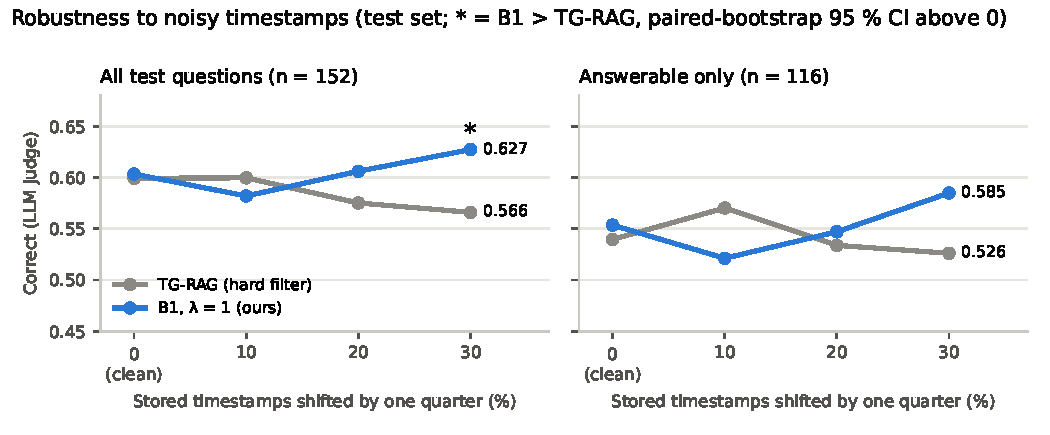
\includegraphics[width=\columnwidth]{figures/robustness_test.pdf}
  \caption{Correct versus the share of stored timestamps shifted by one quarter (test set). A star marks an interval of the difference lying above zero.}
  \label{fig:robust}
\end{figure}

\subsection{Where the methods differ (exploratory)}
On the 116 answerable test questions, B1 changes the retrieved context on 110. It is better than the baseline on 35, worse on 28 and tied on 53; the gains ($+12.90$) and losses ($-11.27$) nearly cancel. By type (Fig.~\ref{fig:types}), B1 helps on multi-time questions (0.522 to 0.596) and single-time multi-keyword questions (0.647 to 0.732). It hurts on single-time multi-company questions (0.697 to 0.516; worse on 13 of 22 answerable ones) and on relative-time questions (0.590 to 0.533). A plausible, untested explanation is that neighbouring-quarter facts help to fill multi-period questions but compete for the fixed context with exact-period facts about the other companies. Questions with no seed under the hard filter occurred on only 2 of 116 answerable test questions (3 of 27 on development); B1 scored 0.458 against 0.000 on them.

\begin{figure}[t]
  \centering
  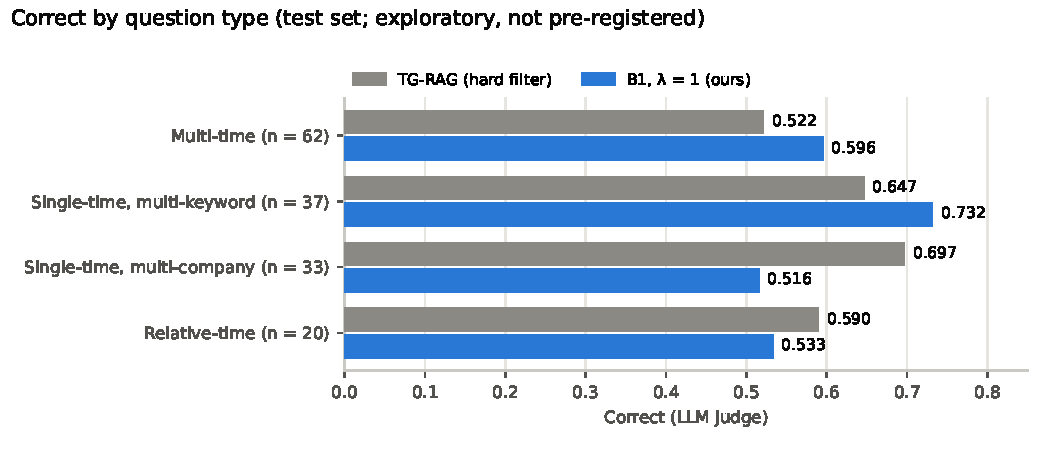
\includegraphics[width=\columnwidth]{figures/per_type_test.pdf}
  \caption{Correct by question type, baseline vs B1 (test set, exploratory).}
  \label{fig:types}
\end{figure}
